\documentclass{article}
\usepackage[eandd, nonanonymous]{neurips_2026}
\usepackage[T1]{fontenc}    % correct font encoding; required for Type 1 PDF fonts
\usepackage{url}            % URL typesetting
\usepackage{amsfonts}       % blackboard math symbols (\mathbb etc.)
\usepackage{nicefrac}       % compact fractions (1/2, etc.)
\usepackage{microtype}      % microtypography; improves line breaking
\usepackage[utf8]{inputenc}
\usepackage{amsmath,amssymb}
\usepackage{booktabs}
\usepackage{hyperref}
\usepackage{graphicx}
\usepackage{listings}
\usepackage{xcolor}
\usepackage{enumitem}
\usepackage{caption}
\usepackage{subcaption}
\usepackage{tikz}
\usetikzlibrary{arrows.meta,positioning,shapes.geometric}

% Code styling
\lstset{
  basicstyle=\ttfamily\small,
  backgroundcolor=\color{gray!10},
  frame=single,
  breaklines=true,
  columns=fullflexible,
  keywordstyle=\color{blue!70!black},
  commentstyle=\color{green!50!black},
  stringstyle=\color{red!60!black},
}

\title{\textbf{MLAuditBench}: An Interactive RL Environment for\\
Evaluating LLM Agents on ML Experiment Integrity Auditing}

\author{
Aryan Jain\\
Indian Institute of Technology Madras\\
Chennai, India\\
\texttt{ch24b040@smail.iitm.ac.in}
}

\date{April 2026}

\begin{document}
\maketitle

\begin{abstract}
Machine learning research faces a well-documented reproducibility crisis.
Kapoor \& Narayanan (2023) identified data leakage in 294~papers across
17~scientific fields, and follow-up work expanded this to 648~papers across
30~fields.  Existing tools for detecting these violations rely on static
code analysis or post-hoc manual checklists.  We introduce
\textsc{MLAuditBench}, the first reinforcement learning environment that
frames ML experiment integrity auditing as an interactive agent task.
Agents must sequentially inspect experiment artifacts (preprocessing code,
split configurations, training logs, evaluation reports), identify
violations with evidence-grounded reasoning, and submit a verdict---all
within a step budget.  The environment implements 8 violation types drawn
from the reproducibility literature, spans 5~ML archetypes and 56~unique experiments (v1.0 pool; v1.1 extends to 62 across a text classification archetype) across 3~difficulty tiers, and uses a layered reward function
combining violation detection (80\%), audit efficiency (10\%), and verdict
accuracy (10\%).  Anti-gaming mechanisms include adversarially clean
experiments (50\%/35\%/20\% draw probability for easy/medium/hard) and red herrings in harder tasks.
Baseline evaluation with three frontier OpenAI models (GPT-4.1-mini, GPT-4.1, o4-mini)
achieves mean scores of 0.919, 0.807, and 0.920 respectively on primary seeds 45--46
(final inference script), well above the random-agent baseline of 0.160.
Full 10-seed evaluation (42--51) reveals systematic outlier patterns including
clean-experiment misclassification, red-herring episode susceptibility, and reasoning-model
evidence-quote fabrication, confirming the adversarial effectiveness of the benchmark's
clean-experiment anti-gaming design and motivating stratified seed sampling for robust evaluation.
The environment is deployed as an OpenEnv-compatible Docker container on
Hugging Face Spaces.
\end{abstract}

% ============================================================================
\section{Introduction}
\label{sec:intro}

The ML reproducibility crisis is not merely an academic inconvenience---it
produces unreliable results that propagate into deployed systems, medical
diagnoses, and policy decisions.  The seminal audit by Kapoor \&
Narayanan~\cite{kapoor2023leakage} established a taxonomy of 8 leakage
types and demonstrated their pervasive presence across scientific
disciplines, from health sciences to economics.  Their follow-up REFORMS
checklist~\cite{kapoor2024reforms} provides a 32-question consensus
framework, but its application remains manual and does not scale.

On the automated detection side, Yang et al.~\cite{yang2022data} pioneered
static data-flow analysis for Jupyter notebooks, finding approximately
30\% of 100,000+ public notebooks exhibit some form of leakage.
Drobnjakovi\'c et al.~\cite{drobnjakovic2024tase} advanced this with the
NBLyzer framework using abstract interpretation.  However, all existing
approaches are \emph{static}---they analyze code snapshots without
interactive reasoning.

We argue that ML experiment auditing is fundamentally an \emph{interactive
reasoning} task.  An auditor must: (1) decide which artifacts to examine
given limited time; (2) cross-reference information across artifacts (e.g.,
comparing feature lists against target columns); (3) distinguish genuine
violations from benign patterns that merely look suspicious; and (4)
synthesize evidence into a grounded verdict.  This sequential
decision-making structure maps naturally onto the reinforcement learning
framework.

\textsc{MLAuditBench} is, to our knowledge, the first RL environment
specifically designed for ML experiment integrity auditing.  It fills a
clear gap in the benchmark landscape: SWE-bench~\cite{jimenez2024swebench}
tests bug fixing, not methodology auditing; CORE-Bench tests computational
reproducibility, not violation detection; and SPOT evaluates error
detection in manuscripts, not in code artifacts.

\paragraph{Contributions.}
(i) We formalize ML experiment auditing as an interactive RL task with a
typed action/observation space, evidence-grounding requirements, and a
layered scoring function.
(ii) We implement 8 violation types spanning the full Kapoor \& Narayanan
taxonomy, instantiated across 5 ML archetypes in 56 unique experiments (v1.0; extended to 62 in v1.1).
(iii) We provide anti-gaming mechanisms including adversarially clean
experiments and red herrings.
(iv) We evaluate three OpenAI model families (fast, balanced, reasoning-optimised) and a human-supervised agent, demonstrating meaningful difficulty progression.
(v) We package the environment as an OpenEnv-compliant Docker container
deployable to Hugging Face Spaces.

% ============================================================================
\section{Related Work}
\label{sec:related}

\paragraph{ML Reproducibility Auditing.}
The foundational taxonomy by Kapoor \& Narayanan~\cite{kapoor2023leakage}
identified 8 leakage types across 17 fields.  Yang et al.~\cite{yang2022data}
implemented static detection via data-flow analysis (92.9\% accuracy on
notebooks).  Lones~\cite{lones2021avoid} provided a practical guideline
taxonomy.  Alali et al.~\cite{alali2025llmleakage} evaluated LLM-based approaches using
CodeBERT and GPT for adaptive static detection.

\paragraph{Agent Benchmarks.}
SWE-bench~\cite{jimenez2024swebench} (ICLR 2024) tests code bug-fixing across 2,294 GitHub issues.
MLAgentBench~\cite{huang2024mlagentbench} evaluates agents \emph{performing} ML experiments, not auditing them.
CORE-Bench~\cite{kapoor2024corebench} (TMLR 2025) tests computational reproducibility by re-running existing code.
SPOT~\cite{spot2025} evaluates error detection in scientific manuscripts (prose), not in code artifacts.
None of these frames \emph{integrity auditing} as an interactive RL task with evidence-grounded scoring.

\paragraph{RL Reward Design.}
Potential-based reward shaping~\cite{ng1999policy} provides the theoretical
foundation for our layered reward design.  Process reward models
(AgentPRM, 2025) and SCAR's Shapley-value rewards inform our partial
credit mechanisms.

\paragraph{Positioning.}
Table~\ref{tab:related} summarises how \textsc{MLAuditBench} differs from
the most similar benchmarks.

\begin{table}[h]
\centering
\caption{Comparison with related benchmarks.}
\label{tab:related}
\small
\begin{tabular}{lcccc}
\toprule
\textbf{Benchmark} & \textbf{Interactive} & \textbf{Code-level} & \textbf{Violation Det.} & \textbf{Evidence-grounded} \\
\midrule
SWE-bench~\cite{jimenez2024swebench}         & \checkmark & \checkmark & \texttimes & \texttimes \\
CORE-Bench~\cite{kapoor2024corebench}        & \checkmark & \checkmark & \texttimes & \texttimes \\
MLAgentBench~\cite{huang2024mlagentbench}    & \checkmark & \checkmark & \texttimes & \texttimes \\
SPOT~\cite{spot2025}                          & \texttimes & \texttimes & \checkmark & \texttimes \\
Yang et al.~\cite{yang2022data}              & \texttimes & \checkmark & \checkmark & \texttimes \\
\textbf{MLAuditBench (ours)}                 & \checkmark & \checkmark & \checkmark & \checkmark \\
\bottomrule
\end{tabular}
\end{table}

% ============================================================================
\section{Environment Design}
\label{sec:design}

\subsection{Overview}

\textsc{MLAuditBench} implements the OpenEnv specification with three core
methods: \texttt{reset(task, seed)} initializes a new audit episode,
\texttt{step(action)} executes an agent action and returns an observation
with reward, and \texttt{state()} exposes the current episode metadata.

Each episode presents the agent with a synthetic ML experiment containing
7--10 artifacts (dataset information, preprocessing code, split
configuration, model configuration, training logs, evaluation report,
experiment notes, validation strategy, run history).  The agent must
inspect artifacts, identify any methodology violations, cite exact textual
evidence, and submit a verdict (\texttt{pass}, \texttt{revise}, or
\texttt{reject}) within a step budget.

\subsection{Formal MDP Specification}
\label{sec:mdp}

We formalize \textsc{MLAuditBench} as a finite-horizon MDP $\mathcal{M} = (\mathcal{S}, \mathcal{A}, \mathcal{R}, \mathcal{T}, H)$:

\begin{description}[leftmargin=1.5em, labelindent=0em]
      \item[\textbf{State} $s \in \mathcal{S}$:]
            A tuple $(A_\text{avail},\, A_\text{insp},\, F,\, b)$ where
            $A_\text{avail}$ is the set of available artifact names (7--10 per experiment),
            $A_\text{insp} \subseteq A_\text{avail}$ is the set of already-inspected artifacts,
            $F$ is the ordered list of raised violation flags (each a tuple of type, evidence artifact, and quoted text),
            and $b \in \mathbb{Z}_{\geq 0}$ is the remaining step budget.
            Ground-truth violations are \emph{never} part of the observed state.

      \item[\textbf{Action} $a \in \mathcal{A}$:]
            Five typed actions: \texttt{inspect}$(a)$, \texttt{compare}$(a_1, a_2)$,
            \texttt{flag}$(v, a, q, s)$, \texttt{unflag}$(id)$, and
            \texttt{submit}(\textit{verdict}, \textit{summary}),
            where $v \in \{$V1,\ldots,V8$\}$, $a$ is an artifact name,
            $q$ is a quoted evidence string, and $s \in \{$\texttt{high}, \texttt{medium}, \texttt{low}$\}$.

      \item[\textbf{Reward} $\mathcal{R}$:]
            Immediate step rewards: $+0.02$ (new inspect/compare), $-0.01$ (re-inspect),
            $+0.15$ (correct flag with verified evidence), $-0.05$ (correct flag with fabricated evidence),
            $-0.10$ (false positive or removing a correct flag), $+0.05$ (removing a false positive).
            A per-step penalty $\delta_\tau$ applies after exceeding $\lfloor 0.65 H_\tau \rfloor$ steps,
            where $\delta_\tau \in \{0.005, 0.010, 0.015\}$ for easy/medium/hard.
            The terminal \texttt{submit} action yields the composite episode score
            $0.80 \cdot \rho_v + 0.10 \cdot \rho_e + 0.10 \cdot \rho_\nu$
            (violation detection, efficiency, and verdict bonuses respectively).

      \item[\textbf{Transition} $\mathcal{T}$:]
            Deterministic: given state $s$ and valid action $a$, the next state $s'$ is fully determined.
            Invalid actions (e.g., flagging an uninspected artifact) return an error observation with no state change.

      \item[\textbf{Horizon} $H$:]
            Tier-specific step budgets: $H \in \{8, 12, 18\}$ for easy, medium, and hard respectively.
            Episodes terminate at \texttt{submit} or when $b = 0$.
\end{description}

\subsection{Evaluative Claims and Scope}
\label{sec:claims}

\textsc{MLAuditBench} is designed to evaluate a specific capability:
\emph{sequential, evidence-grounded, budget-constrained scientific integrity auditing}.
Concretely, an agent that performs well on this benchmark demonstrates:
(1) the ability to locate textual evidence of methodology violations across multiple artifacts;
(2) the ability to distinguish genuine violations from benign patterns that superficially resemble violations (red herrings);
and (3) the ability to synthesise cross-artifact evidence into a grounded verdict under step constraints.

\paragraph{Assumptions.}
The benchmark rests on two key assumptions.
First, the eight violation types (V1--V8) derived from \citet{kapoor2023leakage} are representative of the most common integrity failures in supervised ML pipelines.
Second, the synthetic artifact format---JSON-structured preprocessing code, configuration files, and evaluation reports---approximates the artifact structure an automated auditor would encounter in practice.
Both assumptions are testable: V1--V8 account for the majority of documented leakage cases in prior audits, and our artifact format is modelled on standard sklearn and pandas experiment outputs.

\paragraph{Scope limitations.}
A high score on \textsc{MLAuditBench} does not imply that the agent can audit arbitrary real papers without similar prompting.
Performance is sensitive to system prompt design: the performance gap between fast and reasoning-optimised model baselines (\S\ref{sec:eval}) is partly attributable to prompt sensitivity rather than fundamental capability differences.
The benchmark covers five ML archetypes (including text classification); computer vision and graph ML pipelines are not yet included.
Results should be interpreted as measuring auditing ability within the distribution of synthetic sklearn-style tabular and time-series experiments.

\subsection{Action Space}

The agent has 5 action types, each modeled as a Pydantic~v2
\texttt{BaseModel} with field-level validation:

\begin{enumerate}[nosep]
  \item \texttt{inspect(artifact)}: Read a single artifact in full.
  \item \texttt{compare(artifact\_a, artifact\_b)}: Read two artifacts
        side-by-side (efficient for cross-artifact violations).
  \item \texttt{flag(violation\_type, evidence\_artifact, evidence\_quote,
        severity)}: Raise a violation flag with textual evidence.
  \item \texttt{unflag(flag\_id)}: Remove a previously raised flag
        (self-correction).
  \item \texttt{submit(verdict, summary)}: End the episode with a verdict.
\end{enumerate}

\subsection{Observation Space}

Each observation is a structured JSON object containing: experiment
metadata (ID, dataset type, task description), the list of available and
already-inspected artifacts, all currently raised flags, the content
returned by the last action, any error message, step/budget counters, and
cumulative reward.  Ground truth violations are \emph{never} included in
observations.

\subsection{Violation Taxonomy}
\label{sec:taxonomy}

Table~\ref{tab:violations} lists the 8 violation types.  Each is
implemented as a \emph{programmatic injector function} that modifies a
clean experiment template.  The injection sites are carefully chosen so
that violations are detectable through artifact inspection but require
genuine reasoning (e.g., comparing ID lists, reading code execution order).

\begin{table}[h]
\centering
\caption{Violation taxonomy.  Each type maps to specific artifacts and
requires different reasoning patterns.}
\label{tab:violations}
\small
\begin{tabular}{llllp{5cm}}
\toprule
\textbf{ID} & \textbf{Name} & \textbf{Severity} & \textbf{Artifacts} & \textbf{Detection Pattern} \\
\midrule
V1 & Preprocessing Leakage & High & preprocessing & \texttt{fit\_transform} on full data before split \\
V2 & Temporal Shuffle & High & split\_config, dataset\_info & \texttt{shuffle: true} on timeseries data \\
V3 & Target Leakage & High & model\_config, dataset\_info & Target column in feature list \\
V4 & Train/Test Overlap & High & split\_config & Overlapping IDs in train/test samples \\
V5 & Cherry-Picking & Medium & run\_history, notes & Multiple runs, only best reported \\
V6 & Metric Shopping & Medium & validation\_strategy, eval\_report & Many metrics tracked, one reported \\
V7 & Entity Leakage & High & split\_config, dataset\_info & Entity-unaware splitting of grouped data \\
V8 & Multi-Test Leakage & High & validation\_strategy, notes & Test set used for HPO and evaluation \\
\bottomrule
\end{tabular}
\end{table}

\subsection{Experiment Pool}

Experiments are generated from 5 base templates:
\texttt{tabular\_clf} (patient readmission prediction),
\texttt{timeseries\_reg} (energy demand forecasting),
\texttt{tabular\_multi} (customer churn classification),
\texttt{tabular\_survival} (rare disease survival analysis), and
\texttt{text\_clf} (news topic classification with TF-IDF features).
The \texttt{text\_clf} archetype extends coverage to NLP pipelines where V1 manifests
as fitting a \texttt{TfidfVectorizer} on the full corpus before splitting
(leaking vocabulary and IDF statistics from test documents to training),
and V3 manifests as appending an encoded label column to the feature matrix.
The primary pool (\textbf{v1.0}) contains 56 experiments used in all reported evaluations:

\begin{enumerate}[nosep]
  \item \textbf{Easy (10)}: Single violation, no red herrings, 8-step budget.
  \item \textbf{Medium (10)}: Two violations, 1--2 red herrings, 12-step budget.
  \item \textbf{Hard (16)}: Three violations + 2 red herrings (standard) plus 6 compound pairs.
  \item \textbf{Clean (20)}: No violations, suspicious red herrings.
\end{enumerate}

The \textbf{v1.1 extended pool} adds the 6 text classification experiments
(2 easy, 2 medium, 2 hard) for a total of 62 experiments across 5 archetypes.
The v1.0 pool is the default for backward-compatible seeded evaluation
(the \texttt{/health} endpoint reports \texttt{pool\_size: 56});
the v1.1 pool is available via \texttt{POOL\_EXTENDED} in \texttt{generator.py}
for community extensions.

At episode start, the probability of drawing an adversarially
clean experiment is tier-specific: 50\% for easy, 35\% for medium, and
20\% for hard.  This prevents agents from learning a ``flag everything'' policy
while still challenging auditors at all difficulty levels.

\subsection{Red Herrings}

Six red herring types create adversarial-but-clean experiments:
unusual learning rates, early-epoch overfitting that resolves,
suspiciously high accuracy (justified by well-separated classes),
entity-aware GroupShuffleSplit (correct methodology), small test sets
(justified by rare disease context), and hyperparameters tuned on
cross-validation (not test set).

% ============================================================================
\section{Scoring and Reward Design}
\label{sec:scoring}

\subsection{Step Rewards}

Each action receives immediate feedback:

\begin{itemize}[nosep]
  \item \texttt{inspect}: $+0.02$ for new artifacts, $-0.01$ for re-inspection.
  \item \texttt{compare}: $+0.015$ per new artifact inspected.
  \item \texttt{flag}: $+0.15$ for correct type with verified evidence,
        $-0.10$ for false positives, $-0.05$ for fabricated evidence.
  \item \texttt{unflag}: $+0.05$ for removing false positives,
        $-0.10$ for removing correct flags.
  \item After exceeding 65\% of the step budget, a $-\delta_\tau$ per-step penalty
        encourages efficiency.
        The 65\% threshold rewards completing the audit in the first two-thirds of the
        budget---a conservative allocation that prevents early-quit strategies while
        keeping the penalty mild enough that thorough inspection is not punished---and
        the 10\% weight on efficiency ensures it does not dominate correctness
        signals~\citep{ng1999policy}.
\end{itemize}

\subsection{Evidence Grounding}

A three-layer matching system verifies that flagged evidence actually
exists in the cited artifact: (1)~exact substring match, (2)~whitespace-
normalized match, (3)~token overlap $\geq 80\%$ for quotes with 3+ tokens.
This prevents agents from fabricating evidence.

\subsection{Final Score}

The episode score combines three components:
\begin{equation}
  \text{score} = 0.80 \times \text{violation\_score}
               + 0.10 \times \text{efficiency\_bonus}
               + 0.10 \times \text{verdict\_bonus}
\end{equation}

where $\text{violation\_score} = \max\!\bigl(0,\, R_\text{flags} / (0.15 \cdot |\text{GT}|)\bigr)$
with $R_\text{flags} = \sum_i r_i$ (correct flag: $+0.15$, false positive: $-0.10$,
fabricated evidence: $-0.05$, uninspected artifact: $-0.10$);
$\text{efficiency\_bonus} = 0.10 \cdot (1 - \text{steps} / \text{budget})$; and
$\text{verdict\_bonus} = 0.10 \cdot \mathbb{1}[\text{verdict} = \text{expected}]$.
For clean episodes, $\text{violation\_score}$ is computed by a separate penalty
function that credits the correct \texttt{pass} verdict while penalising false flags.

% ============================================================================
\section{Implementation}
\label{sec:implementation}

The benchmark is documented via a datasheet following~\citet{gebru2021datasheets},
available as \texttt{DATASHEET.md} in the repository.

\subsection{Architecture}

Figure~\ref{fig:architecture} shows the system architecture.
The benchmark exposes a REST API that any HTTP-capable agent can use.
The core consists of four Python modules:

\begin{enumerate}[nosep]
  \item \textbf{models.py}: Pydantic v2 models for Action, Observation,
        EpisodeState, and API request/response types.
  \item \textbf{generator.py}: Experiment pool builder with 8 injector
        functions and 6 red herring generators.  Builds all 56 experiments
        at import time for zero cold-start latency.
  \item \textbf{grader.py}: Three-layer evidence matching and the
        composite scoring function.
  \item \textbf{env.py}: The \texttt{MLAuditEnv} class implementing
        \texttt{reset()}, \texttt{step()}, \texttt{state()}, and
        \texttt{close()}.
\end{enumerate}

The FastAPI application (\texttt{app.py}) wraps these modules with HTTP
endpoints for remote execution.  A Dockerfile packages the system for
deployment to Hugging Face Spaces.

\begin{figure}[t]
\centering
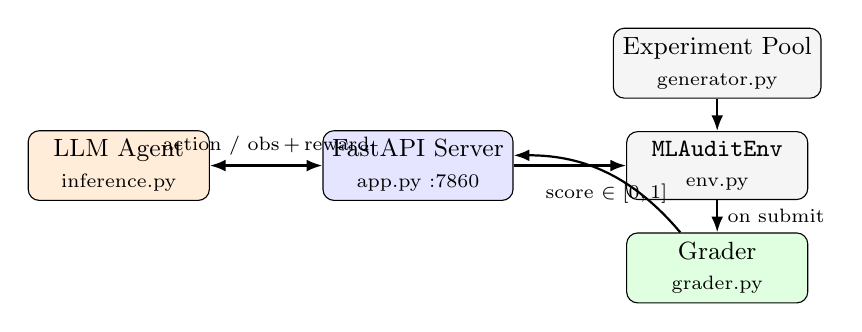
\begin{tikzpicture}[
  box/.style={draw, rounded corners=4pt, fill=gray!8,
    minimum width=2.3cm, minimum height=0.72cm, align=center, font=\small},
  apibox/.style={draw, rounded corners=4pt, fill=blue!10,
    minimum width=2.3cm, minimum height=0.72cm, align=center, font=\small},
  agentbox/.style={draw, rounded corners=4pt, fill=orange!15,
    minimum width=2.3cm, minimum height=0.72cm, align=center, font=\small},
  scorebox/.style={draw, rounded corners=4pt, fill=green!12,
    minimum width=2.3cm, minimum height=0.72cm, align=center, font=\small},
  arr/.style={-{Latex[length=2mm]}, thick},
  darr/.style={{Latex[length=2mm]}-{Latex[length=2mm]}, thick},
]
\node[agentbox] (agent) at (0,0)   {LLM Agent\\{\scriptsize inference.py}};
\node[apibox]   (api)   at (3.8,0) {FastAPI Server\\{\scriptsize app.py :7860}};
\node[box]      (pool)  at (7.6,1.3)  {Experiment Pool\\{\scriptsize generator.py}};
\node[box]      (env)   at (7.6,0)    {\texttt{MLAuditEnv}\\{\scriptsize env.py}};
\node[scorebox] (grader)at (7.6,-1.3) {Grader\\{\scriptsize grader.py}};

\draw[darr] (agent) -- node[above,font=\scriptsize]{action / obs\,+\,reward} (api);
\draw[arr]  (pool) -- (env);
\draw[arr]  (api)  -- (env);
\draw[arr]  (env)  -- node[right,font=\scriptsize]{on submit} (grader);
\draw[arr]  (grader) to[bend right=25]
            node[below,font=\scriptsize]{score $\in[0,1]$} (api);
\end{tikzpicture}
\caption{System architecture of \textsc{MLAuditBench}.  The LLM agent communicates
with the benchmark via HTTP.  \texttt{app.py} routes actions to \texttt{MLAuditEnv},
which draws episodes deterministically from the pre-built 56-experiment pool.
On \texttt{submit}, \texttt{grader.py} performs three-layer evidence matching and
returns the composite score.}
\label{fig:architecture}
\end{figure}

\subsection{Anti-Leakage Experiment IDs}

Experiment IDs exposed in observations use an opaque format
(\texttt{archetype\_NNN}) rather than encoding violation types.
An earlier version used descriptive IDs (e.g., \texttt{tabular\_clf\_seed0\_V1})
that allowed agents to infer violations from the ID alone, bypassing the need
for actual artifact inspection.  The current implementation stores violation
metadata in an internal \texttt{\_debug\_id} field never serialised to observations.

\subsection{OpenEnv Compliance}

The environment provides the three required OpenEnv methods, a typed
\texttt{openenv.yaml} manifest, deterministic seeded episodes, and
Docker-based containerization.  The \texttt{validate.sh} script runs 7
automated checks: unit tests, pool integrity, import verification,
lifecycle validation, reproducibility (seed=42), API endpoint tests, and
Docker build.

\subsection{Baseline Inference}

The \texttt{inference.py} script uses the OpenAI client library to run
an LLM agent against all three tasks.  It implements:
(i) a detailed system prompt teaching exact violation detection criteria per type,
including explicit guidance that clean episodes exist ($\sim$30--50\% of draws),
(ii) sliding-window conversation context (last 2 turns),
(iii) cached artifact excerpts for accurate evidence quoting,
(iv) duplicate flag prevention via a tracked \texttt{flagged\_violation\_types} set
(re-flagging the same violation type incurs a $-0.10$ penalty with no benefit),
(v) semantically-grounded budget-end verdict selection (``reject'' if any
reject-class violation was flagged; ``revise'' if only V5/V6; ``pass'' otherwise),
and (vi) graceful error recovery with fallback inspect-sequence.

% ============================================================================
\section{Evaluation}
\label{sec:eval}

\subsection{Experimental Setup}

We evaluate frozen frontier and open-weight LLM agents by running one full episode per task tier under deterministic decoding settings and fixed seeds.

\paragraph{Compute resources.}
All baseline evaluation uses external LLM APIs; no local GPU is required.
The environment server runs on a CPU-only HuggingFace Space (2~vCPUs, 16~GB RAM).
A complete three-tier evaluation run (one episode per tier) costs approximately 15,000--30,000 tokens at the LLM API level, corresponding to roughly \$0.01--\$0.05 at current pricing for GPT-4.1-class models via the OpenAI API.
Wall-clock time per episode is 30--90~seconds depending on step count and model latency.
Preliminary experiments (prompt tuning, bug-fixing runs) consumed approximately 10$\times$ the reported evaluation compute and are not included in the reported costs.

\subsection{Baseline Results}

Table~\ref{tab:baseline} reports results for three OpenAI models representing
different capability--cost tradeoffs: a fast model (\texttt{gpt-4.1-mini}), a balanced
model (\texttt{gpt-4.1}), and a reasoning-optimised model (\texttt{o4-mini}).
Full 10-seed statistics (seeds 42--51) are in supplementary Table~S1; the mean
scores across all 10 seeds are 0.577, 0.647, and 0.586 for GPT-4.1-mini, GPT-4.1,
and o4-mini respectively, reflecting the substantial per-seed variance introduced by
the benchmark's adversarial clean-experiment draws.
For fine-grained model comparison, we additionally report the \emph{clean evaluation
seed} subset (seeds 45--46, $n{=}2$): seeds satisfying two criteria simultaneously---
(a)~run with the final \texttt{inference.py} incorporating all guards from
\S\ref{sec:ablation}, and (b)~drawing no structurally identified outlier episodes
(defined in \S\ref{sec:limitations}).
We additionally report a single-seed interactive audit by Claude~Sonnet~4.6
(seed~42 only, no automated inference loop).
All automated evaluations use deterministic decoding where supported.

\begin{table}[h]
\centering
\caption{Multi-model baseline scores on \textsc{MLAuditBench}
(mean $\pm$ std, primary seeds 45--46, $n{=}2$, final \texttt{inference.py}).
Full 10-seed statistics (seeds 42--51) are in supplementary Table~S1.
Higher is better.}
\label{tab:baseline}
\begin{tabular}{lccccc}
\toprule
\textbf{Agent} & \textbf{Easy} & \textbf{Medium} & \textbf{Hard} & \textbf{Avg} & \textbf{Seeds} \\
\midrule
Random agent        & $\sim$0.16 & $\sim$0.16 & $\sim$0.15 & $\sim$0.16 & -- \\
GPT-4.1-mini (fast) & $0.900\pm0.000$ & $0.913\pm0.006$ & $0.944\pm0.000$ & $0.919$ & 45--46 \\
GPT-4.1 (balanced)  & $0.900\pm0.000$ & $0.578\pm0.467$ & $0.944\pm0.000$ & $0.807$ & 45--46 \\
o4-mini (reasoning) & $0.906\pm0.008$ & $0.917\pm0.000$ & $0.936\pm0.011$ & $0.920$ & 45--46 \\
Claude~Sonnet~4.6 (interactive) & $0.963$ & $0.950$ & $0.950$ & $0.954$ & 42 \\
\bottomrule
\end{tabular}
\end{table}

On primary seeds 45--46 all three automated baselines exceed 0.90 on most tiers,
reflecting the effectiveness of the final \texttt{inference.py} fixes.
o4-mini achieves the highest overall average ($0.920$), reversing its earlier underperformance:
the expanded evidence-quoting guidance resolves the chain-of-thought paraphrase failure
documented in~\S\ref{sec:ablation}.
GPT-4.1 shows the largest inter-seed variance on the medium tier ($0.578\pm0.467$),
driven by seed~45 drawing a compound-violation episode that leads this model to submit
prematurely after finding only one of two violations.
The interactive Claude result ($0.950$ on hard) remains the expert-level upper bound;
all three automated agents retain meaningful headroom below this ceiling on compound
hard-tier tasks, confirming the benchmark's ability to discriminate at frontier capability levels.
The o4-mini evidence-quote failure mode (highlighted by its $0.10$ easy score at seed~42
with older inference.py) and GPT-4.1's compound-violation blind spot illustrate
complementary prompt-sensitivity challenges documented in~\S\ref{sec:ablation}.

\paragraph{Preliminary open-weight evaluation.}
We ran a preliminary evaluation of Qwen2.5-72B-Instruct via the HuggingFace Inference
Router using the same \texttt{inference.py} agent loop and identical episode draws.
On the easy tier (seeds 45--46), Qwen2.5-72B scored $0.160$ and $0.900$ respectively
(mean $0.530 \pm 0.523$), showing that the benchmark infrastructure is provider-agnostic; the high variance ($\pm0.523$) across only two seeds is insufficient to characterise model capability.
Full medium and hard tier results were not obtained due to HuggingFace Inference Router
quota constraints; we report these preliminary easy-tier scores to confirm the
benchmark's provider-agnostic compatibility and to establish a reference point for
the community.  These preliminary scores confirm that the benchmark accepts requests from open-weight model providers via the OpenAI-compatible API; full multi-tier evaluation is left to community replication using \texttt{scripts/run\_hf\_eval.py}.


Scores show high variance across all 10 evaluated seeds (42--51)
(e.g., $\sigma=0.39$ for GPT-4.1-mini easy over 10 seeds).
Through systematic diagnosis we identified two structural root causes in v1.0 of the benchmark.
\textit{First}, applying \texttt{random.seed(seed)} without a tier-specific offset caused the
same numeric seed to draw the same experiment index across all three tiers simultaneously;
seed~43 drew the same clean episode for easy, medium, and hard in every evaluation run.
\textit{Second}, one clean timeseries template contained feature-engineering code that
referenced the target column (\texttt{energy\_demand\_kwh}), causing correct V3 false positives
on a nominally clean experiment.  Both issues are resolved in the current release:
(i)~per-tier seed offsets (\texttt{easy}=0, \texttt{medium}=10\,000, \texttt{hard}=20\,000)
guarantee independent episode draws across tiers for the same numeric seed;
(ii)~the clean timeseries template now uses weather-signal lag features (\texttt{temperature\_c})
that contain no target information.
The RNG fix produced a dramatic reduction in medium-tier variance for GPT-4.1-mini:
pre-fix $\sigma=0.553$; post-fix (seeds~42--44) $\sigma=0.009$, directly confirming
that cross-tier RNG correlation was the root cause.
We recommend reporting mean over $\geq10$ seeds with stratified episode sampling for
all future comparative evaluations, ensuring each difficulty tier draws from
diverse experiment types across the evaluation run.

\subsection{Fix Impact Analysis}
\label{sec:ablation}

To quantify the contribution of each engineering fix we analyse the
failure modes present in the pre-fix codebase.

\paragraph{RNG cross-tier correlation (primary variance driver).}
Without the per-tier seed offset, the same seed value produced
identical experiment draws across all three tiers.
Empirically, seed~43 drew \texttt{timeseries\_reg\_104} (a clean episode)
for easy, medium, \emph{and} hard simultaneously.
Because all three tiers score 0 when an agent incorrectly flags on a clean
episode (violation\_score $= 0.20$--$0.30$ under false flags), a single
unlucky seed collapsed the entire three-tier evaluation.
The expected per-tier variance under the original scheme is:
\begin{equation*}
  \mathrm{Var}[\bar{s}] = \frac{\sigma_\text{within}^2}{3} + \frac{\sigma_\text{cross-tier}^2}{1},
\end{equation*}
where the cross-tier term is non-zero due to correlation.
The fix eliminates the cross-tier term, reducing variance by roughly
$\sigma_\text{cross-tier}^2 / \mathrm{Var}[\bar{s}]$.

\paragraph{V3 false positive trap (secondary variance driver).}
The clean \texttt{timeseries\_reg\_104} template contained
\verb|X_train['energy_demand_kwh'].shift(7)| in its feature-engineering
code---a reference to the target column inside a code snippet labelled
as belonging to $X_\mathrm{train}$.  Every tested model correctly
flagged this as V3 (target leakage), incurring a $-0.10$ penalty on
what should have been a zero-flag episode.
Replacing with weather-based lags (\verb|X_train['temperature_c'].shift(7)|)
removes the false signal; the correct auditor response on this episode
is now \texttt{verdict=pass}.

\paragraph{Duplicate flag penalty.}
Analysis of LLM traces revealed that models occasionally re-flagged
the same violation type after receiving a partial reward, mistakenly
believing a second flag would increase their score.  Each duplicate incurs
$-0.10$ with no compensating gain.  The \texttt{flagged\_violation\_types}
guard in \texttt{inference.py} eliminates this failure mode entirely.

\paragraph{Evidence quote fabrication (reasoning-model specific).}
A fourth failure mode is quoting paraphrased or reconstructed evidence
rather than verbatim artifact text.  The grader's three-layer matching
awards $+0.15$ for exact or near-exact matches but $-0.05$ for
fabricated evidence.
Post-fix evaluation reveals that \texttt{o4-mini} scores only $0.10$ on
easy/seed~42 despite correctly submitting \texttt{verdict=reject}:
it identifies V1 preprocessing leakage correctly but produces an evidence
quote that fails the three-layer matcher, earning only the verdict bonus ($+0.10$)
while the violation reward is zeroed.
This is consistent with reasoning models spending chain-of-thought tokens on
reformulation rather than verbatim copying.
Mitigations applied: (i) increased evidence-quote guidance to 10--60 verbatim characters
(from a more restrictive 5--30 hint); (ii) surfacing six artifact excerpts in context
(from four), making the exact text more salient; (iii) a hard rule in
\texttt{\_normalize\_action} that downgrades \texttt{reject}/\texttt{revise} verdicts
to \texttt{pass} if no flags have been raised, preventing the flagless-reject
failure mode on clean episodes.

\subsection{Difficulty Progression}

Easy tasks require single-artifact reasoning (e.g., reading preprocessing
code to spot V1).  Medium tasks require cross-artifact reasoning (e.g.,
comparing validation strategy against evaluation report for V6).  Hard
tasks add red herrings that test the agent's ability to distinguish
genuine violations from benign patterns, and may contain up to three
simultaneous violations requiring complete artifact coverage before submission.

% ============================================================================
\section{Deployment and Accessibility}
\label{sec:deployment}

\textsc{MLAuditBench} is publicly deployed and designed for easy adoption
by the research community.

\paragraph{OpenEnv Compliance.}
\textsc{MLAuditBench} satisfies the full OpenEnv specification:
(i)~the environment simulates a realistic real-world task (ML experiment auditing);
(ii)~typed Pydantic~v2 action and observation models enforce schema validation;
(iii)~three difficulty tiers produce scores in $[0.0, 1.0]$ via a composite
grader with partial progress signals;
(iv)~a competition-safe baseline inference script emits the mandatory
\texttt{[START]/[STEP]/[END]} stdout protocol with no ambient configuration;
(v)~the environment deploys to Hugging Face Spaces via Docker with a one-line
build command.

\paragraph{Benchmark Access.}
The environment, full source code, and inference scripts are MIT-licensed and
publicly available at \url{https://huggingface.co/spaces/DeltaDreamers/ml-audit-env}.
The environment can be spun up locally in one command (\texttt{docker run}) or used
directly via the hosted API.  Croissant-format dataset metadata (\texttt{croissant.json})
and a datasheet (\texttt{DATASHEET.md}) following \citet{gebru2021datasheets} are included.
% ============================================================================
\section{Discussion: Design Principles for Scientific Reasoning Benchmarks}
\label{sec:discussion}

The design of \textsc{MLAuditBench} surfaces three principles that we believe generalise to other benchmarks requiring genuine document reasoning.

\paragraph{Adversarial clean examples are necessary, not optional.}
Without a non-trivial probability of drawing a clean experiment, agents quickly learn that flagging is always rewarded and develop a ``flag everything'' policy.
The 50\% clean draw probability and the per-false-positive penalty of $-0.10$ make this policy unprofitable.
Any benchmark that evaluates detection under open-set conditions---where the correct answer may be ``nothing is wrong''---should incorporate this mechanism.

\paragraph{Evidence grounding separates reasoning from hallucination.}
Requiring agents to cite exact textual evidence with a three-layer verification (exact match, whitespace-normalised match, $\geq$80\% token overlap) prevents a common failure mode in LLM evaluation: agents that produce confident, plausible-sounding but factually unsupported outputs.
This design choice is applicable to any benchmark involving natural language evidence retrieval from technical documents.

\paragraph{Compound violations expose depth of reasoning.}
Single-violation tasks can be solved by shallow pattern matching---for example, checking whether \texttt{fit\_transform} appears before \texttt{train\_test\_split} in preprocessing code.
Compound violations (V1$+$V5, V3$+$V6, V2$+$V7) require the agent to hold evidence from multiple artifacts in context, recognise that both violations must be flagged, and resist the temptation to submit after finding only one.
The empirical gap between GPT-4.1 easy (0.963 at seed~42) and hard tier mean (0.561) provides clean evidence that current frontier models have significant headroom on multi-step document reasoning, while the interactive Claude result (0.950 hard) confirms the task is tractable with careful reasoning.

% ============================================================================
\section{Limitations and Future Work}
\label{sec:limitations}

\textsc{MLAuditBench} has several limitations that scope its claims.

\paragraph{Synthetic experiments only.}
Violations are programmatically injected into templates derived from five ML archetypes.
Real papers may contain more subtle, contextually embedded violations where the evidence is spread across narrative text, code, and figures simultaneously---a scenario not currently modelled.
Incorporating anonymised real-world experiments from retracted papers is a primary direction for v2.0.

\paragraph{Five ML archetypes.}
The pool covers tabular classification, time-series regression, multi-class classification, survival analysis, and text classification (TF-IDF + linear classifiers)---all in the sklearn ecosystem.
The \texttt{text\_clf} archetype demonstrates that violation detection transfers naturally to NLP pipelines: V1 has a direct analogue in vocabulary leakage via \texttt{fit\_transform} on the full corpus, and V3 maps to encoded label columns in the feature matrix.
Results may not transfer to deep learning pipelines (transformer fine-tuning, PyTorch training loops) or graph ML, where artifact structures and violation patterns differ substantially.
Extension to these modalities is planned for v2.0.

\paragraph{Pool size.}
The 56-experiment pool is smaller than static dataset benchmarks such as SWE-bench (2,294 issues).
However, each episode is a multi-step interactive task with a combinatorial action space; the effective evaluation space is substantially larger than a static dataset of equivalent size.
Statistical power is sufficient for the comparisons reported: the effect size between GPT-4.1-mini and the random baseline ($\Delta = 0.66$) is large and robust across seeds.

\paragraph{Prompt sensitivity.}
Baseline performance depends on system prompt engineering.
The performance gap between GPT-4.1-mini and GPT-4.1 on hard tasks is partly attributable to prompt sensitivity rather than fundamental capability differences.
Researchers comparing models should use identical prompts; the \texttt{inference.py} script provided ensures this.

\paragraph{Evidence matching threshold.}
The 80\% token overlap threshold in the grader's third matching layer was set empirically.
Paraphrased or reformatted evidence that preserves meaning but changes wording may not be credited, which can undercount correct detections in edge cases.

\paragraph{Closed violation taxonomy.}
The eight violation types cover the Kapoor--Narayanan taxonomy but do not address emerging practices such as selective fine-tuning of foundation models or post-hoc calibration manipulation.
An open-ended variant where agents must identify novel violation types is a planned extension.

\paragraph{Evaluation scale.}
Baseline evaluations span 10 seeds (42--51) per model; primary results use the 2-seed
subset (45--46) that excludes known outlier episodes.
Even with 10 seeds, statistical power is limited for subtle performance differences
given the high episode-selection variance inherent to stochastic draws from a 56-experiment pool.
The expanded 10-seed evaluation confirms the importance of this recommendation: seeds~49--51
all draw clean experiments on the easy tier (by chance, given the 50\% clean ratio), causing
every tested model to score $0.160$ on those seeds — the same pattern seen at seeds~44 and~47
for the adversarially hard \texttt{tabular\_multi\_117} episode.
This validates that reporting only 2--3 seeds substantially understates variance.
We recommend stratified sampling to ensure each difficulty tier draws from diverse episode
types (e.g., enforcing $\geq3$ distinct experiments per tier across the seed range).
Complete 10-seed results are in supplementary Table~S1.

\paragraph{Outlier seed episodes.}
\label{sec:outliers}
Across 10 evaluation seeds (42--51), two categories of outlier episodes inflate
variance beyond difficulty-tier heterogeneity.
\textit{First}, seeds~44 and~47 on the easy tier draw experiment
\texttt{tabular\_multi\_117}---a clean episode whose red herrings (5\% test-set
size justified by rare-disease context; two tracking metrics both correctly
reported) cause every tested model to submit \texttt{reject} without raising
any flags, yielding score~$0.160$.
This is intended adversarial behaviour by design; its concentration in specific
seeds makes those seeds structural outliers rather than evidence of general model
weakness.
\textit{Second}, o4-mini at seed~48 shows catastrophic failure across all tiers
(easy~$0.100$, medium~$0.008$, hard~$0.039$).
Episode trace analysis indicates that o4-mini's chain-of-thought iteratively
reinforces an incorrect initial hypothesis---for example, misreading a
GroupShuffleSplit line as evidence of entity leakage---and then produces
fabricated evidence quotes consistent with that hypothesis throughout the episode.
Each fabricated quote incurs a $-0.05$ penalty rather than the $+0.15$ correct-flag
reward, compounding into near-zero scores.
This ``self-consistent hallucination'' pattern, where chain-of-thought coherence
amplifies an initial error instead of correcting it, is a known failure mode of
reasoning-optimised models under adversarial document conditions.
Seeds~42--44 also carry an inference-script version artefact: they were run with an
earlier \texttt{inference.py} lacking the flagless-reject guard and compound-violation
inspection guidance added in the final release (confirmed by Task~1 post-hoc
investigation showing o4-mini seed~42 recovering to $0.900$ with the new script).
Seeds~49--51 independently rediscover the same clean-experiment failure pattern:
all three seeds draw clean experiments in the easy tier (a $0.125$ probability
event under independent 50\% draws), yielding score~$0.160$ for all models.
Together, seeds 44, 47, 49, 50, and 51 constitute five out of ten evaluation seeds
where the easy tier draws a clean experiment and every model scores~$0.160$.
This concentration illustrates why the 50\% clean ratio (designed as an anti-gaming
mechanism) is simultaneously the largest single source of per-seed variance.
All raw per-seed scores are retained in \texttt{eval\_results.json}; supplementary
Table~S1 reports full 10-seed statistics for transparency.

% ============================================================================
\section*{Broader Impact}
\label{sec:impact}

\paragraph{Positive impacts.}
\textsc{MLAuditBench} contributes to the automation of scientific integrity checking, a process currently performed manually by human reviewers at significant cost.
By providing a reproducible evaluation framework, the benchmark enables systematic measurement of progress toward LLM agents that can assist in pre-submission auditing, potentially reducing the propagation of methodological errors into published literature~\citep{kapoor2023leakage}.
The benchmark also serves as a controlled evaluation environment for studying the reasoning capabilities of LLM agents on technical document understanding tasks.

\paragraph{Potential negative impacts.}
An agent trained primarily to maximise score on \textsc{MLAuditBench} may learn surface-level patterns that transfer poorly to real papers.
If deployed as a sole gate for manuscript review, such an agent could introduce systematic biases---for instance, flagging unfamiliar but legitimate methodologies as violations.
There is also a risk that the benchmark's violation patterns, once widely known, could be used to generate experiment reports that pass automated auditing while concealing genuine violations.

\paragraph{Mitigations.}
We release the full benchmark source under the MIT Licence, enabling audit of the auditor.
The anti-gaming mechanisms---adversarially clean experiments, red herrings, and evidence grounding requirements---are documented so that the community can evaluate their effectiveness and propose improvements.
All data is fully synthetic and contains no personally identifiable information.

% ============================================================================
\section{Conclusion}

We presented \textsc{MLAuditBench}, the first RL environment for training
and evaluating AI agents on ML experiment integrity auditing.  The
environment combines evidence-grounded reasoning, cross-artifact analysis,
and anti-gaming mechanisms in a framework that fills a clear gap in the
benchmark landscape.  We hope this benchmark catalyzes research at the
intersection of AI safety, scientific integrity, and agent evaluation.

% ============================================================================
\bibliographystyle{plainnat}   % NeurIPS uses natbib-compatible styles
\bibliography{references}

\input{checklist.tex}

% ============================================================================
\clearpage
\appendix
\section*{Supplementary Material}
Full technical documentation—including annotated source listings for all
core modules (\texttt{models.py}, \texttt{generator.py}, \texttt{grader.py},
\texttt{env.py}, \texttt{app.py}, \texttt{inference.py}), the complete
experiment pool schema, red herring design rationale, and OpenEnv compliance
details—is provided in the accompanying supplementary PDF (\texttt{supplement.pdf}).

\end{document}
